%==============================================================================
% ETHASL - Template for student projects at the ASL
% 2013.10: Péter Fankhauser
% This template is based on the IMRT Latex template by Eric A. Mueller.
%==============================================================================

\documentclass[10pt,oneside,a4paper]{report}

\usepackage{pdfpages}
\usepackage{float}
\usepackage[demo]{graphicx}
%\usepackage{caption}
\usepackage{subcaption}
%\usepackage{subfigure} 
%\usepackage{subfig}
\usepackage{unicode-math}
\usepackage{amsmath}
\usepackage{amssymb}
\usepackage{tabularx}
\usepackage{array}
\usepackage{eqexpl}

% ETHASL package
% TODO Choose options according to your project
% som/bt/st/mt: Studies on Mechatronics, Bachelor Thesis, Semester Thesis, Master Thesis
% fs/hs: Spring term, Autumn term
% german/english: German/English
\usepackage[st,hs,english]{packages/ethasl}

% Activate for german language
%\usepackage{german}
%\usepackage{ae}

%%%%%%%%%%%%%%%%%%%%%%%%%%%%%%%%%%%%%%%%%%%%%%%%%%%%%%%%%%%%%%%%%%%%%%%%%%%%%%%
% LaTeX preamble
%%%%%%%%%%%%%%%%%%%%%%%%%%%%%%%%%%%%%%%%%%%%%%%%%%%%%%%%%%%%%%%%%%%%%%%%%%%%%%%
% Encoding settings
\usepackage[utf8]{inputenc}
\usepackage[OT1]{fontenc}

% Paper size
\usepackage{a4}

% Headings
\usepackage{fancyhdr}

% More symbols
\usepackage{textcomp}\usepackage{gensymb}

% Math support for Times font
%\usepackage{txfonts}

% ISO date
\usepackage[english]{isodate}

% Multi column
\usepackage{multicol}

% Figures
\usepackage{graphicx}

% Subfigures (obsolete)
\usepackage{subfig}

% Bibliography
\usepackage[numbers]{natbib}

% Nicer tables
\usepackage{booktabs}
\usepackage{array}
\usepackage{multirow}

% Colors
\usepackage{color}
\usepackage{colortbl}
\definecolor{black}{rgb}{0,0,0}
\definecolor{white}{rgb}{1,1,1}
\definecolor{darkred}{rgb}{0.5,0,0}
\definecolor{darkgreen}{rgb}{0,0.5,0}
\definecolor{darkblue}{rgb}{0,0,0.5}

% Additional math functionality
\usepackage{amsmath}
\usepackage{amssymb}

% Nice fractions
\usepackage{nicefrac}

% Upper case greek letters
\usepackage{upgreek}

% ISO math notation
\usepackage{isomath}
\renewcommand{\vec}{\vectorsym}
\newcommand{\mat}{\matrixsym}

% Units
\usepackage{units}

% Rotated objects
\usepackage{rotating}

% Indent
\setlength{\parindent}{0em}

% Include PDF pages
\usepackage{pdfpages}
\includepdfset{pages={-}, frame=true, pagecommand={\thispagestyle{fancy}}}

% Headings
\rhead[\thepage]{\nouppercase{\rightmark}}
\lhead[\nouppercase{\leftmark}]{\thepage}
\cfoot{}

% Gantt chart
\usepackage{pgfgantt}

% Links (last package)
\PassOptionsToPackage{hyphens}{url}\usepackage{hyperref}

% Clever references (has to be loaded after hyperref)
\usepackage{cleveref}


%%%%%%%%%%%%%%%%%%%%%%%%%%%%%%%%%%%%%%%%%%%%%%%%%%%%%%%%%%%%%%%%%%%%%%%%%%%%%%%
% Title page
%%%%%%%%%%%%%%%%%%%%%%%%%%%%%%%%%%%%%%%%%%%%%%%%%%%%%%%%%%%%%%%%%%%%%%%%%%%%%%%
\begin{document}

% TODO Add your title
\title{Crop Row Detection Leading to Autonomous Navigation of a Laser-based Weeding Robot}
%\subtitle{bla bla bla}

% TODO Add name of the authors
\studentA{Roxane Mérat}
%\studentB{Student 2}
% \studentC{Student 3}

% TODO Add name of the supervisors
\supervisionA{Cornelius von Einem}
\supervisionB{Patrick Barton}
%\supervisionC{Supervisor C}

% TODO Change if necessary
\projectYear{2022} % This year
%\projectYear{\advance\year by -1 \the\year\advance\year by 1} % Last year

\maketitle
\pagestyle{plain}
\pagenumbering{roman}

%%%%%%%%%%%%%%%%%%%%%%%%%%%%%%%%%%%%%%%%%%%%%%%%%%%%%%%%%%%%%%%%%%%%%%%%%%%%%%%
% Declaration of originality
%%%%%%%%%%%%%%%%%%%%%%%%%%%%%%%%%%%%%%%%%%%%%%%%%%%%%%%%%%%%%%%%%%%%%%%%%%%%%%%
\pagestyle{empty}
% TODO Modify placeholders in declaration.tex
%% TODO Add title, student first/last name, supervisor first/last name.

\section*{Declaration of Originality}

\vspace{1cm}

I hereby declare that the written work I have submitted entitled

\vspace{0.5cm}

% TODO Add title
\textbf{Your Project Title}

\vspace{0.5cm}

is original work which I alone have authored and which is written in my own words.\footnote{Co-authored work: The signatures of all authors are required. Each signature attests to the originality of the entire piece of written work in its final form.}

\vspace{1cm}

\textbf{Author(s)}

\vspace{0.5cm}

\begin{tabular}{ p{5cm} p{5cm} }
% TODO Add student first/last name
  First name & Last name \\
\end{tabular}

\vspace{0.5cm}

\textbf{Student supervisor(s)}

\vspace{0.5cm}

\begin{tabular}{ p{5cm} p{5cm} }
% TODO Add supervisor first/last name
  First name & Last name \\
\end{tabular}

\vspace{0.5cm}

\textbf{Supervising lecturer}

\vspace{0.5cm}

\begin{tabular}{ p{5cm} p{5cm} }
  Roland & Siegwart \\
\end{tabular}

\vspace{1cm}

With the signature I declare that I have been informed regarding normal academic citation rules and that I have read and understood the information on 'Citation etiquette' (\url{https://www.ethz.ch/content/dam/ethz/main/education/rechtliches-abschluesse/leistungskontrollen/plagiarism-citationetiquette.pdf}).
The citation conventions usual to the discipline in question here have been respected.

\vspace{0.5cm}

The above written work may be tested electronically for plagiarism.

\vspace{4cm}

\begin{tabular}{ p{5cm} p{1cm} p{5cm} }
  \cline{1-1} \cline{3-3}
  Place and date & & Signature \\
\end{tabular}


\includepdf[pagecommand={}]{Report/chapters/declaration-originality.pdf}


%%%%%%%%%%%%%%%%%%%%%%%%%%%%%%%%%%%%%%%%%%%%%%%%%%%%%%%%%%%%%%%%%%%%%%%%%%%%%%%
% Table on contents
%%%%%%%%%%%%%%%%%%%%%%%%%%%%%%%%%%%%%%%%%%%%%%%%%%%%%%%%%%%%%%%%%%%%%%%%%%%%%%%

% Table of Contents depth (TODO change if necessary)
\setcounter{tocdepth}{2}

\tableofcontents
\cleardoublepage

%%%%%%%%%%%%%%%%%%%%%%%%%%%%%%%%%%%%%%%%%%%%%%%%%%%%%%%%%%%%%%%%%%%%%%%%%%%%%%%
% Chapters standard
%%%%%%%%%%%%%%%%%%%%%%%%%%%%%%%%%%%%%%%%%%%%%%%%%%%%%%%%%%%%%%%%%%%%%%%%%%%%%%%

\input{chapters/preface}
\cleardoublepage

\chapter*{Symbols}
\label{sec:symbols}
\addcontentsline{toc}{chapter}{Symbols}
%\chapter*{Symbolverzeichnis}
%\label{sec:symbole}
%\addcontentsline{toc}{chapter}{Symbolverzeichnis}

\section*{Symbols}
%\section*{Symbole}

\begin{tabbing}
 \hspace*{1.6cm} \= \kill
  $\rho$ \> distance of a point from the origin \\[0.5ex] 
  $\theta$  \>  angle between the point and the positive x-axis  					
\end{tabbing}

\section*{Indices}
%\section*{Indizes}
\begin{tabbing}
 \hspace*{1.6cm}  \= \kill
 $x$ \> x axis \\[0.5ex]
 $y$ \> y axis \\[0.5ex]
\end{tabbing}

\section*{Acronyms and Abbreviations}
%\section*{Akronyme und Abkürzungen}
\begin{tabbing}
 \hspace*{1.6cm}  \= \kill
 CNN \> Convolutional Neural Networks \\[0.5ex]
 LiDAR \> Light Detection And Ranging \\[0.5ex]
 IMU \> Inertial Measurement Unit \\[0.5ex]
 UAV \> Unmanned Aerial Vehicle \\[0.5ex]
 CRBD \> Crop Row Benchmark Dataset  \\[0.5ex]
 CRDA \> Crop Row Detection Accuracy \\[0.5ex]
 GNSS \>  Global Navigation Satellite System   \\[0.5ex]
 RANSAC \> Random Sample Consensus  \\[0.5ex]
 VO \> Visual Odometry  \\[0.5ex]


\end{tabbing}
\cleardoublepage

%%%%%%%%%%%%%%%%%%%%%%%%%%%%%%%%%%%%%%%%%%%%%%%%%%%%%%%%%%%%%%%%%%%%%%%%%%%%%%%
% Chapters custom
%%%%%%%%%%%%%%%%%%%%%%%%%%%%%%%%%%%%%%%%%%%%%%%%%%%%%%%%%%%%%%%%%%%%%%%%%%%%%%%
\pagestyle{fancy}
\pagenumbering{arabic}


% TODO Add your own chapters here
\chapter{Introduction}
\label{sec:introduction}
%\chapter{Einleitung}
%\label{sec:einleitung}

 One of the major challenges facing the agricultural industry today is the problem of weeds. Traditional methods of weed removal include large amounts of herbicides, which are harmful to the environment, or manual labor, which is extremely time-consuming and tiring. To address this issue, Caterra, a project under the Crop Science Laboratory of ETH Zurich, is developing a robotic system that uses a laser module to automatically eliminate weeds. \\

This project requires the rover robot to navigate autonomously. For now, most agricultural robots use GNSS to accomplish this task. However, GNSS-based navigation is prone to many problems:
\begin{itemize}
    \item It relies on a fixed infrastructure, such as ground-based reference stations, which may not be available or practical in remote agricultural areas.
    \item The field conditions, weather, and other environmental factors can affect the accuracy of the GNSS signals and cause errors in navigation.
    \item The field environment is constantly changing, with crops growing and harvested, making it difficult for the robot to accurately map and navigate the area.
\end{itemize}

In general, GNSS can provide a rough location of the robot in an agricultural field, but it is not the most robust and reliable solution for autonomous navigation. The need for a more robust method with instant feedback is necessary. Machine vision approaches, specifically visual odometry using an RGB camera, have been extensively researched as an alternative. These methods provide greater robustness and precision and are cost-effective and easy to maintain.

The detection of crop rows is a key aspect in enabling proprioception in agricultural robots and can also be used for other important applications such as crop counting, yield prediction, and field mapping. However, due to the variability in crop type, growth stage, and environmental conditions, detecting crop rows is a challenging task. Many image processing techniques that have been developed are often limited in their ability to detect crop rows robustly under different conditions and their need for a significant amount of manual tuning, and there is a pressing need to develop more robust, adaptable, and automated image processing techniques that can effectively handle the variability of crop rows and environmental conditions. \\


To develop such an algorithm, we have integrated three key principles: Hough transform to extract the main lines from the image, vanishing point calculation to eliminate outliers, and RANSAC to obtain more precise information about the center of each crop row while taking into consideration the fundamental characteristics of crop rows. This will enable further research on the autonomous navigation capabilities of the rover robot.

\begin{figure}[H]
   \centering
   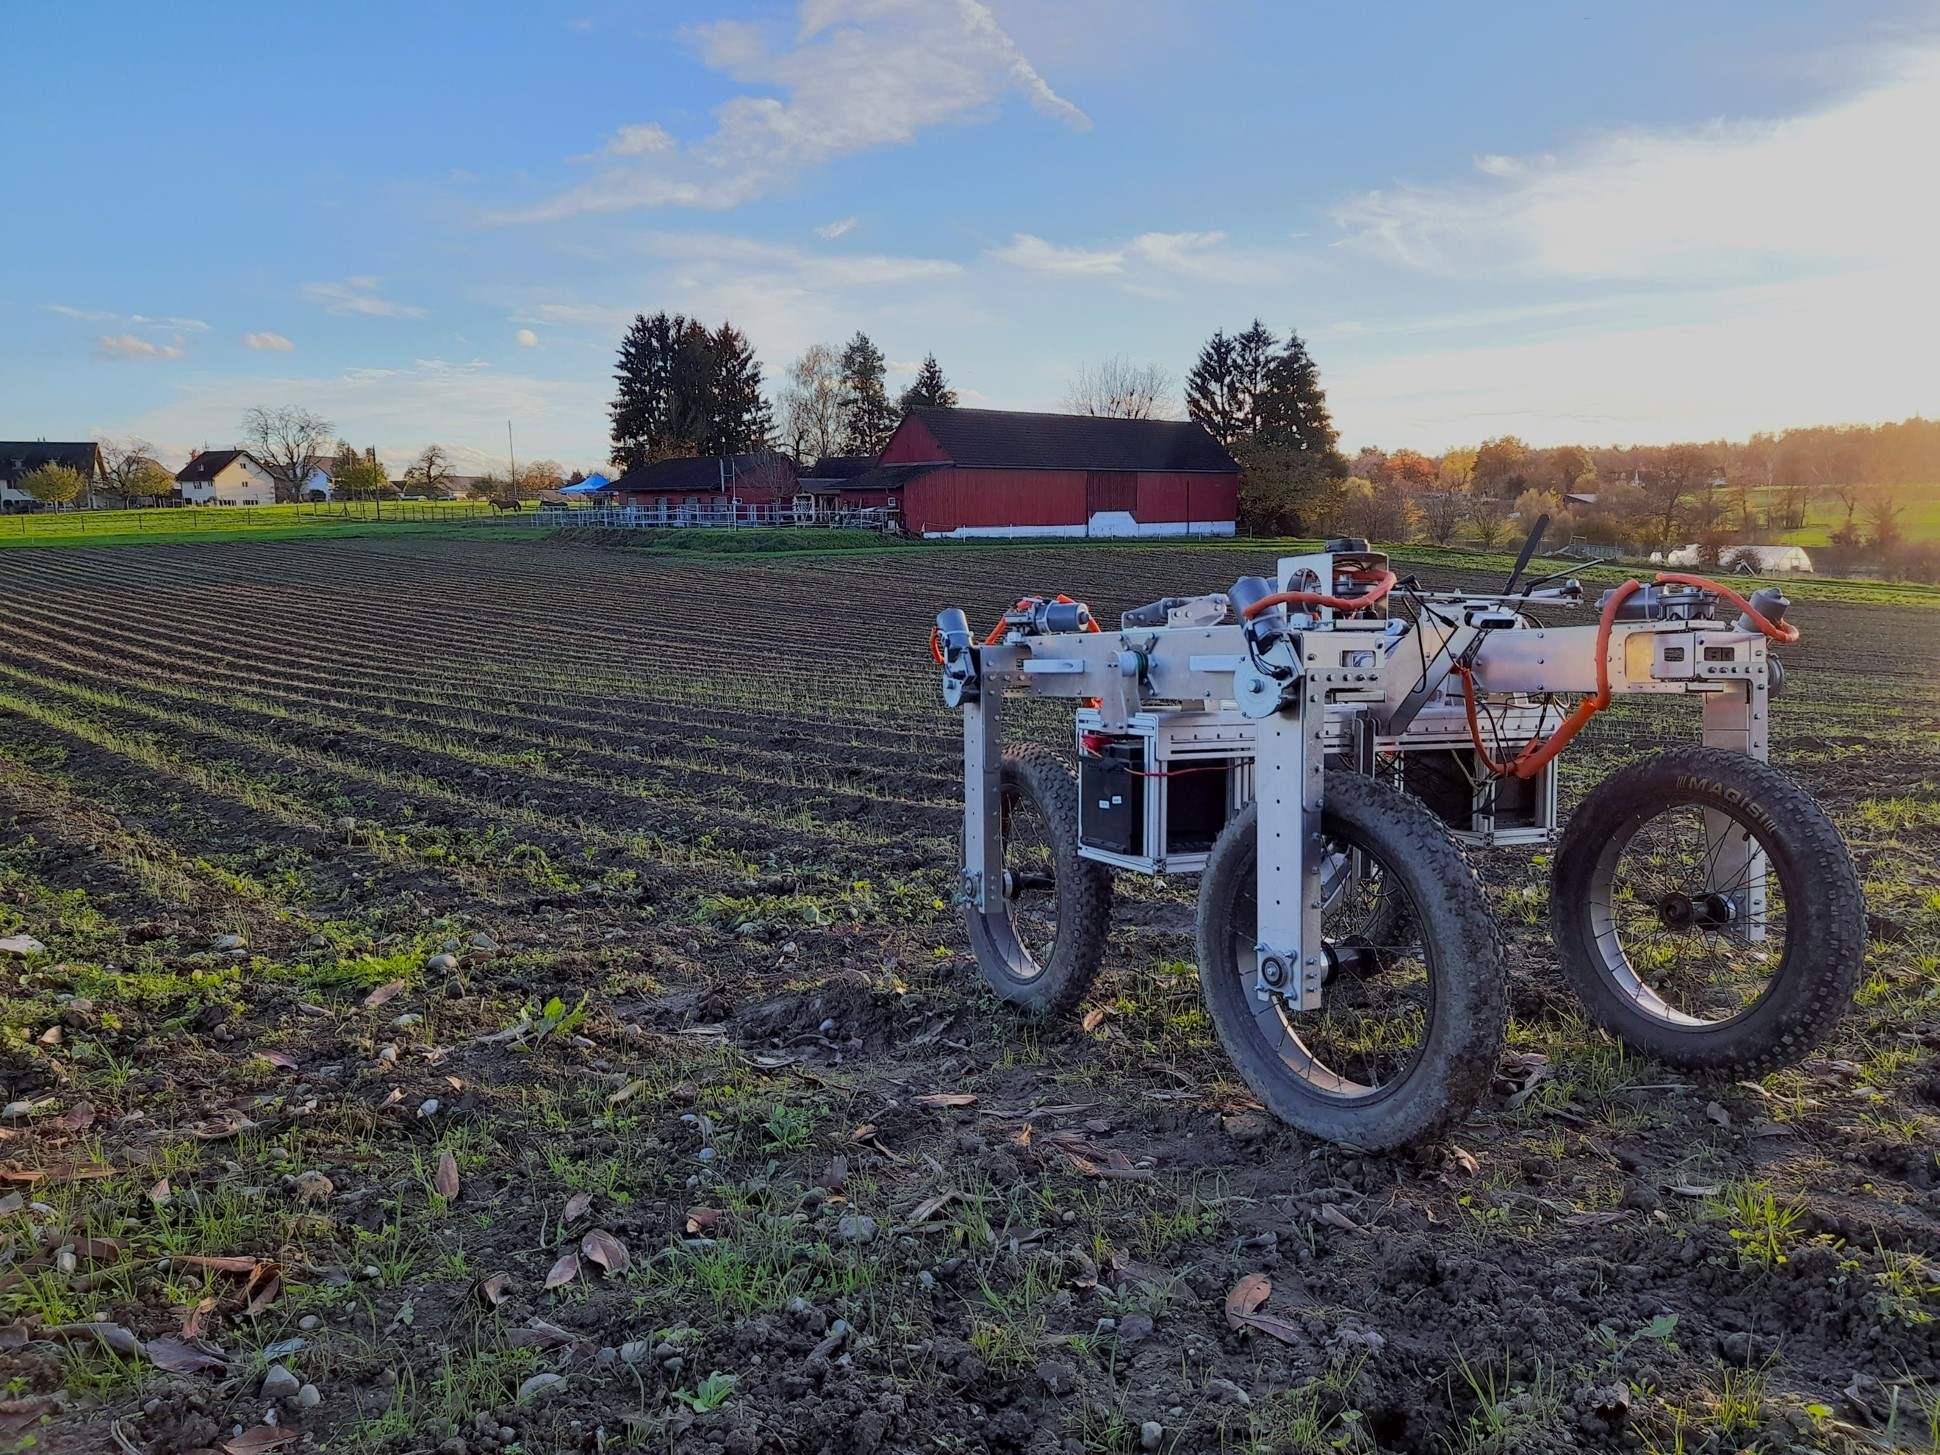
\includegraphics[width=0.75\textwidth]{Report/images/caterracoolrobot.jpg}
   \caption{Caterra's agricultural robot}
   \label{pics:coolrobot}
\end{figure}
\cleardoublepage
\chapter{Overview of previous work in the field of crop row detection}
\label{sec:latexumg}

A lot of research has been done to autonomously detect crop rows using computer vision.The main approaches are LiDAR based techniques, CNN's, and more classical Machine Vision approaches. \\

\section{LiDAR based techniques}


As \citet{AgricultureLiDARZhang} and \citet{LiDARCHangingplantgrowth} have shown,  height information can be used to detect crop rows. However, while the detection of crops during the late period is successful with LiDAR, this technique is not reliable when it comes to the detection of tiny plants, in the early stages of development. The cost of LiDAR sensors is also high and is not suitable for large-scale configuration of agricultural vehicles.   

\section{Convolutional Neural Networks}
CNN can also be used to process images of crop rows and detect rows in new images (\citet{CNN1}, \citet{thesisDOHA}, \citet{DeepLearning2}). However, deep learning methods are limited by the available datasets. As the appearance of the crop row varies a lot depending on the type of crop, the growth stage, the environmental condition and the weather condition, the required dataset must be huge. In our case, we would also need images taken from the same height and angle as our rover.  Today, such large-scaled datasets are not available, and acquiring our own would be very difficult, time consuming, and should be done at various seasons of the year and on various crops.

\section{Classical Machine Vision approach}


\subsection{Segmentation}

To distinguish crops from the background, segmentation is usually performed using color index-based segmentation followed by threshold-based segmentation (\cite{VEGEIDX}). 

Color index segmentation is widely used in agricultural image processing, the most common being the Excess Green Index (ExG, \cite{ExgreenIdx}), the Color Index of Vegetative Extraction (CIVE, \cite{CIVE}) and the normalized difference vegetation index (NDVI, \cite{NDVI}). Post-processed, the new gray image has higher-intensity pixels in place of the pixels.

Once the image is grayscaled, it is usually binarized. The selection of the threshold has to be very well tuned. 
A common technique is to use Otsu thresholding (\citet{4310076}), which autonomously finds a threshold that maximizes the variance between the foreground (the vegetation) and the background. This works by iterating through all possible threshold values and for each one, calculating the variance (how much the intensities in each group differ from the group's mean intensity) between the two groups of pixels. \\

As these techniques are highly sensitive to light changes, some use learning-based segmentation, mainly deep learning, to obtain the best segmentation values (\citet{deepLforSeg}). 

Since no large dataset for vegetation segmentation was accessible, here a threshold-independent segmentation method using color clustering was developed, which will be described later.

\subsection{Line-detection}

Once the vegetation is segmented and a binary image has been computed, a line detection algorithm is necessary to extract crop rows. Currently, the most commonly used line-fitting techniques are the Hough transform, the least squares method, and the Random Sample Consensus. 

\subsubsection{Hough Transform}
\label{subsubsection:HT}

Used to detect lines, circles, or more complex shapes, the Hough transform converts the pixel space to a parameter space, as illustrated in Fig. \ref{fig:HOUGHTRANS}
In the case of line detection, each line in the image is described by the parameters $\rho$  and $\theta$ as such : 
\begin{equation}
\rho(\theta) = x_{0} \cdot \cos{\theta} + y_{0} \cdot \sin{\theta} 
\end{equation}




The Hough space is defined as a graph with abscissa $\theta$ and $\rho$, so each point ($\theta_{i}$, $\rho_{i}$) describes a line in the image space. Once each pixel of an image is mapped to the Hough space, the intensity values at a certain point ($\theta_{i}$, $\rho_{i}$) will be higher when this point describes a prominent line in the image pixels plane. 

This technique is one of the most widely used (\citet{HTRTTracking}) but, on its own, it is not sufficient to detect crop rows robustly. It is highly sensitive to noise (lightning, shading, bushiness, various stages of growth), which requires substantial manual tuning and can lead to false detection of lines. In a region of high weed pressure, many lines are feasible. It is also computationally expensive and difficult to use for real-time applications. 

\begin{figure}[H]
\begin{minipage}{0.5\columnwidth}

\includegraphics[width=\columnwidth,height=4cm]{Report/images/ImageProcesses/HoughProcess/VegeMask.png}
\\[3mm]

\includegraphics[width=\columnwidth,height=4cm]{Report/images/ImageProcesses/HoughProcess/HoughLineDrawned.png}
\captionsetup{justification=centering}
\subcaption{Line detected in Image Space by the Hough Process}
\end{minipage}
\hspace{1cm}
\begin{minipage}{0.8\columnwidth}
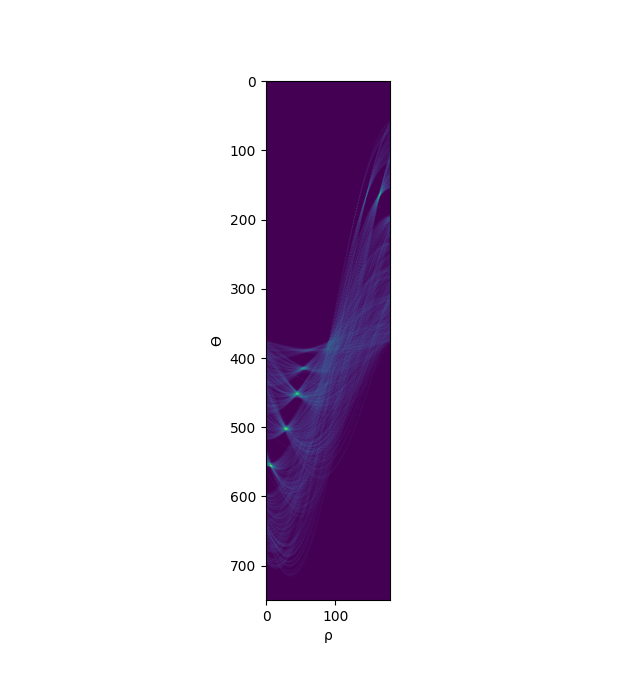
\includegraphics[width=\columnwidth,height=83mm]{Report/images/ImageProcesses/HoughProcess/HoughAcc.png}
\captionsetup{justification=centering}
\subcaption{ Accumulator in the Hough Space\\ $\rho$ [pixel count], $\theta$ [rad]}

\end{minipage}
\hspace{1cm}
\caption{Illustration Hough process}        
\label{fig:HOUGHTRANS}

\end{figure}


\subsubsection{Least square}

\citet{LeastSquares2} and \citet{LeastSquares} use least squares to fit the different rows of crops. Although faster and more robust to weeds, this technique requires prior knowledge to fit the template, such as the number of crop rows to be detected, the expected location of each crop row, and the area to be explored in the image. \\


\subsubsection{RANSAC}

RANSAC (RANdom SAmple Consensus) is an iterative algorithm for estimating the parameters of a mathematical model from a set of observed data that contains outliers (i.e. data that do not fit the model). Here, it is used for line fitting, and the model is defined by the slope and a point on the line. The basic idea behind it is to randomly select a subset of the data points (2 inliers are selected for line fitting) and use them to estimate the parameters of the model. The remaining points (the outliers) are then used to test the validity of the model. This process is repeated multiple times, and the model with the most inliers is chosen as the final solution. The inliers are the points that fall within a certain distance threshold from the line, and the outliers are the points that fall outside of this threshold. RANSAC is a robust algorithm that can handle outliers and still find the correct solution - in our case, it will eliminate weeds or vegetation in between crops. It is faster than the complete Hough transform method and, thus, more adapted for real-time applications.
https://www.overleaf.com/project/6397556aaa04834b75ffb811#

However, as with the least squares method, some prior information on crop rows is necessary: \citet{RANSACbase} based their RANSAC process on a skeleton of the row features. \\ \\ \\ \\

\begin{figure}[H]
\centering
\begin{subfigure}{0.49\textwidth}
    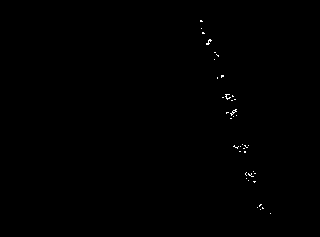
\includegraphics[width=\textwidth]{Report/images/masked images _ransac.png}
    \label{fig:singlelinemask}
\end{subfigure}
\begin{subfigure}{0.49\textwidth}%
    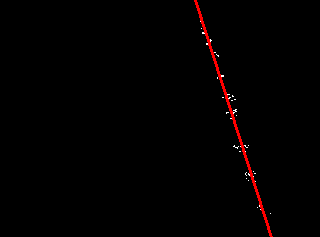
\includegraphics[width=\textwidth]{Report/images/masked images _ransacfitted.png}
    \label{fig:ransacfitsingline}
\end{subfigure}

\caption{Results of the RANSAC algorithm for line fitting}
\end{figure}
\label{pics: Ransacmasking}

\vspace{20mm}

In this project, an algorithm is developed that combines different methods to make each of them more robust and efficient. Hough transform is used as a preprocessing step to calculate the vanishing point and the approximate location of crops, the vanishing point is used to detect outlier lines not parallel in world coordinates, and RANSAC is used to detect the center of each crop rows. 








\cleardoublepage
\chapter{Methodology}
\label{sec:latexumg}

\section{Global description of the algorithm}
\label{sec:gliederung}

The Algorithm can be divided into four main steps : 
\begin{enumerate}
    \item Preprocessing : segments the vegetation from its background
    \item Hough Transform : extracts the main lines of the image  
    \item Outlier line detection : using the vanishing point, eliminates the lines that are not crossing at that point and replaces them with the next most prominent lines in the image
    \item RANSAC : using points around mask corresponding to the regions around the lines previously detected, calculates the center of the crops
\end{enumerate}

The complete algorithm can be visualized in Fig. \ref{pics:AlgoFlowChart}. \\

The algorithm works on single images or sequences of images. As the Hough transform is computationally expensive, the algorithm doesn't use it at each frame : at the end of the RANSAC process, the region of the crops for the next frame is updated : as low changed between each frame was considered, the region where the crops were on the previous frame is used as a reference. As long as the crops detected are considered "valid", only the RANSAC process is runned again, the vanishing point staying the same. 

Frames are considered invalid if two crops are too close to each other, if two crops have too similar an angle, if a crop has an angle too close to the horizon, if there are too few vegetation pixels in the area of the crops detected in the previous frame, or if the frame number is a multiple of K (K can be adapted according to the precision needed).

\begin{figure}
   \centering
   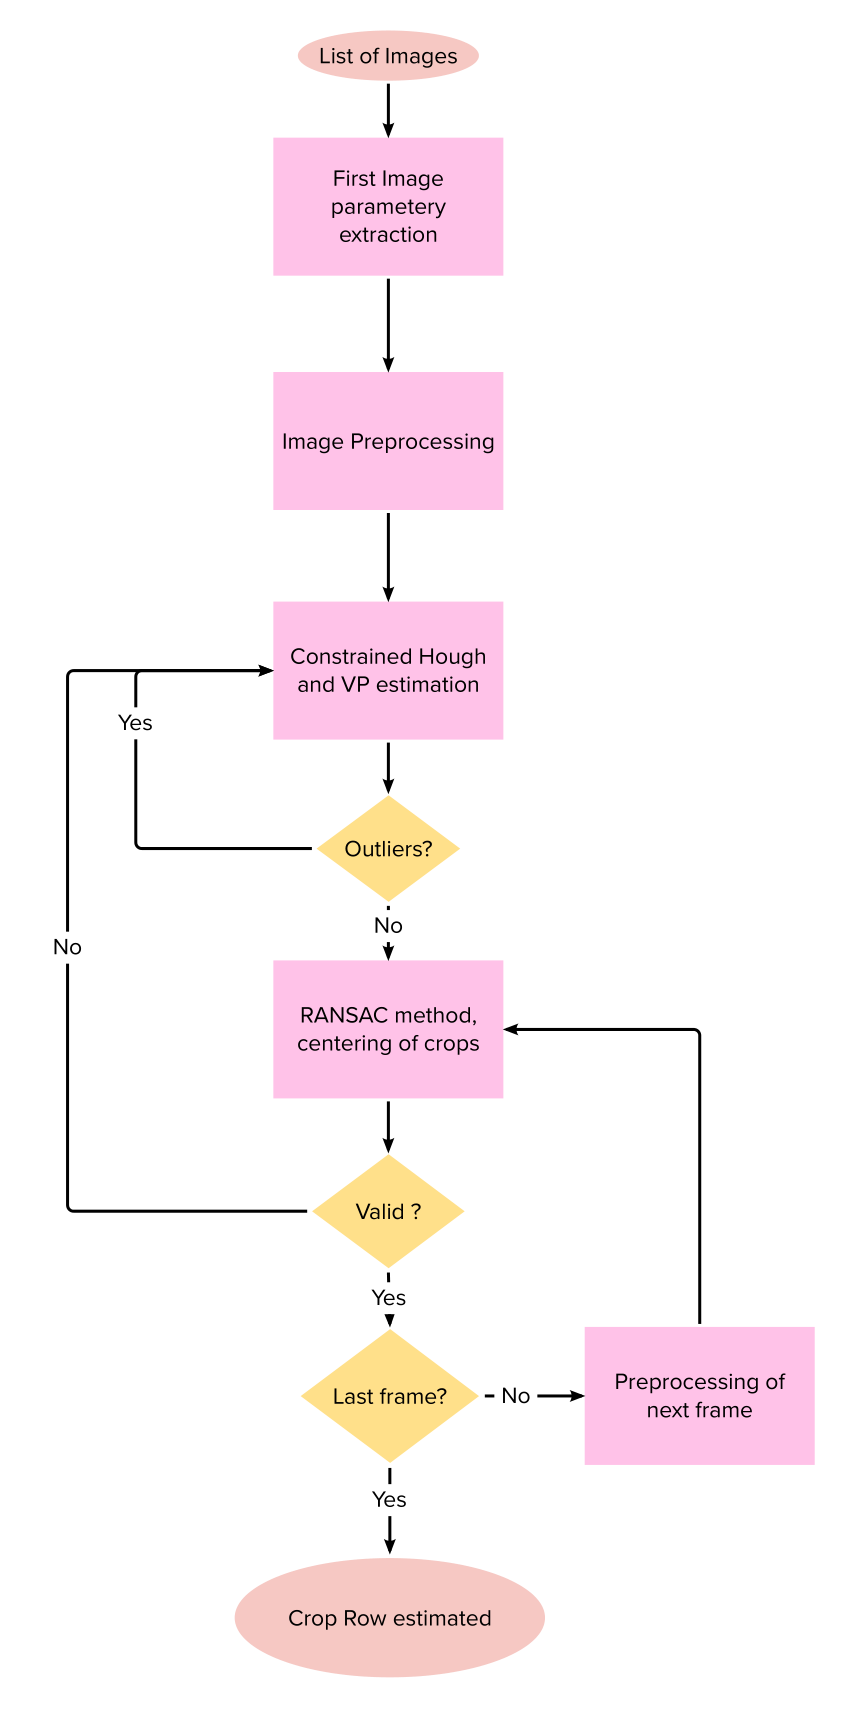
\includegraphics[width=0.75\textwidth]{Report/images/FlowCharts/Algo14_01_2023-01-16_13-58-50.png}
   \caption{Flowchart of the Algorithm}
   \label{pics:AlgoFlowChart}
\end{figure}

\section{Image Preprocessing : sky extraction and vegetation segmentation}
\label{sec:gliederung}

The Preprocessing part of the algorithm serves many purposes:
\begin{enumerate}
    \item Extracts and resizes images
    \item Removes the sky
    \item Removes the extremely bushy regions
    \item Clusters the main colours and extracts the greenest one
    \item Masks the image using a custom threshold on this colour 
    \item Depending on the density of the segmented vegetation, calculates edges of the image or keeps the entire image before proceeding with the first Hough Transform
    \end{enumerate}

\subsubsection{Sky Removal}

This step reduces the Region of Interest of our image to speed up the algorithm. Results are shown in Fig. \ref{eq:my_equation} It consists of three main parts: 

\begin{itemize} 
  \item Laplacian Calculation and thresholding : the Laplacian (the second derivative of the image) is calculated to identify edges and fine details. Pixels with low Laplacian are kept -these are the areas of small changes, which should represent the sky.
  \item Horizon Line Detection : after median filter is applied per column, the first pixels of each column with a high level of change are memorized.
  \item Elimination of non-sky regions : Starting from the top row, the algorithm eliminates horizontal rows until it finds a row where a line is composed of less than 50\% sky (low Laplacian pixels).
\end{itemize}

\begin{figure}[H]
\centering
\begin{subfigure}{0.49\textwidth}
    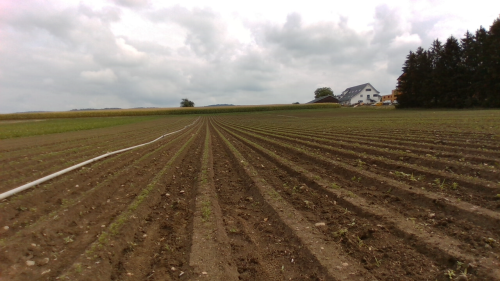
\includegraphics[width=\textwidth]{Report/images/IMGWITHSKY.png}
    \label{fig:first}
\end{subfigure}
\begin{subfigure}{0.49\textwidth}%
    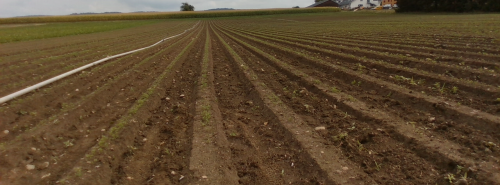
\includegraphics[width=\textwidth]{Report/images/IMGNOSKY.png}
    \label{fig:second}
\end{subfigure}
\caption{Results of the sky removal algorithm}
\end{figure}
\label{pics: Vegewithandwithoutsky}

\subsubsection{Colour Clustering, vegetation colour extraction}

As the vegetation’s colour varies a lot depending on the lighting, a threshold for the vegetation index isn't robust enough. 

K clusters of colors are created by counting the number of pixels with the same color in an image. The color with the highest pixel count is grouped with all other colors that have a difference in LAB space less than a certain threshold. This process is repeated for the second highest pixel count color, and so on, until at max $l$ clusters are formed (cf tables \ref{appendix:hyperparam}, stops before if all pixels have been classified). The outcome can be seen in figure \ref{pics:ColourClus}.

\begin{figure}[H]
   \centering
   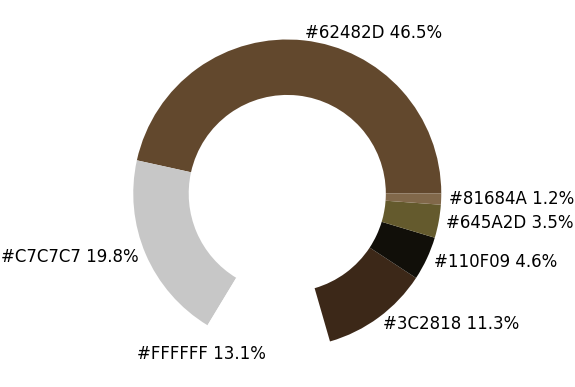
\includegraphics[width=0.75\textwidth]{images/donut.png}
   \caption{Visualisation of the clustered colour}
   \label{pics:ColourClus}
\end{figure}

The algorithm compares the clustered colors to the color with the norm closest  to [0, 255, 0] (lime in RGB space) in LAB space. This color is used to create a mask for the image and segment the vegetation by retaining all pixels with a LAB space difference under a certain threshold. \\

%TODO : maybe do tab at the end with all the hyperparameters values ?

In the video mode of the algorithm, the assumption is made that the color of the vegetation does not change much throughout the video. The reference vegetation color is calculated in frame 0. Although the reference color does not change, the threshold used during masking does, as the goal is to maintain the same level of information throughout the video (the ratio of 1-pixels to 0-pixels in the binary image being used to define "information."). The threshold value is adapted based on this ratio: if the ratio is smaller than the one in frame 0, the threshold is increased, and vice versa. This allows the algorithm to quickly segment the vegetation while maintaining the same level of information throughout the process. Recalculating the reference color at each frame is possible, but this technique has shown satisfactory results, is less computationally expensive, and is more stable. 

\begin{figure}[H]
\centering
\begin{subfigure}{0.49\textwidth}
    
\includegraphics[width=\textwidth]{Report/images/VEGEIMG5.png}
    \label{fig:first}
\end{subfigure}
\begin{subfigure}{0.49\textwidth}%
    
\includegraphics[width=\textwidth]{Report/images/VEGEIMG500.png}
    \label{fig:second}
\end{subfigure}
\caption{Vegetation Image of frame 5 and frame 500}
\end{figure}
\label{pics: Vegestablealongtime}

\subsubsection{Bushy Region Removal}

The image is eroded by a kernel proportional to its size. This new image is then subtracted from the original image. Results can be shown in Fig. \ref{pics: bushyremoval} 

\begin{figure}[H]
\centering
\begin{subfigure}{0.49\textwidth}
    
\includegraphics[width=\textwidth]{Report/images/IMGALLBUSHES.png}
    \label{fig:first}
\end{subfigure}
\begin{subfigure}{0.49\textwidth}%
    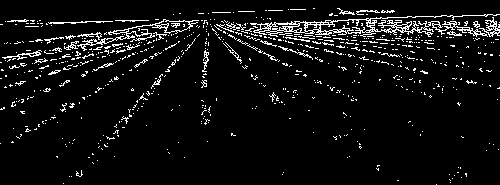
\includegraphics[width=\textwidth]{Report/images/IMGNOBUSHES.png}
    \label{fig:second}
\end{subfigure}
\caption{Erosion of the bushy regions}
\end{figure}
\label{pics: bushyremoval}

\section{First approximation of the crop rows : Hough Transform}
\label{sec:gliederung}

Our interest in the Hough Transform is two-fold : the lines are both used to calculate the vanishing point and to isolate the regions where the crop rows should be found in the RANSAC part of the algorithm. \\

\begin{figure}[h!]
\begin{minipage}{0.48\columnwidth}

\includegraphics[width=\columnwidth,height=4cm]{Report/images/beforelineremoval.png.png}
\\[3mm]

\includegraphics[width=\columnwidth,height=4cm]{Report/images/afterlineremoval.png}
\end{minipage}
\hspace{0.15\columnwidth}
\begin{minipage}{0.3\columnwidth}
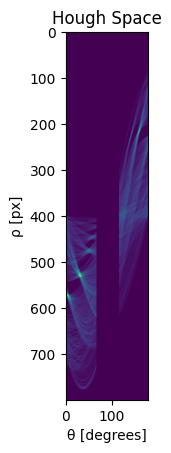
\includegraphics[width=\columnwidth,height=83mm]{Report/images/ImageProcesses/HoughSpacePerso/HTwithlabelconstraint.png}

\end{minipage}
\caption{Illustration of the Hough process}
\label{pics:diffHT}

\end{figure}


The Hough Transform described in section \ref{subsubsection:HT} finds all the lines in the image with values in the accumulator greater than a certain threshold.

To ensure that the lines detected are spaced by a minimum threshold and no angle is the same, the algorithm implemented in this project uses a slightly different Hough transform.\\

Depending on the density of the vegetation, either the entire binary image or the edges of the binary image are taken (if the vegetation pixels are more then 10\% of the entire pixels) to accelerate the process.

Instead of using a threshold to take all lines, the N-maximums of the Hough space are extracted, where N is the number of desired rows. N is set to a defined number but the algorithm  can decrease this number if not enough lines satisfying the "crop conditions" are detected (as further explained in section \ref{sec:VPdet}). This approach allows the algorithm to be independent of a threshold.

When in Hough space, the maximum values to be selected must satisfy the following conditions : 
\begin{enumerate}
    \item No crops should have the same angle : this is done by putting a 0-band in the Hough space around each previously detected angle (cf Fig \ref{pics:diffHT}).
    \item Each 1-pixels should be used only once, to detect a line of a single row. This is done by masking the surroundings of where a line has been detected (cf Fig. \ref{pics:diffHT}). 
\end{enumerate}

Deletion of lines and angles is done iteratively.\\

This process ensures no crops are detected twice, but doesn't prevent detecting lines that are not going towards the vanishing point. 




\section{Vanishing Point Calculation and outliers elimination}
\label{sec:VPdet}

\begin{figure}[H]
   \centering
   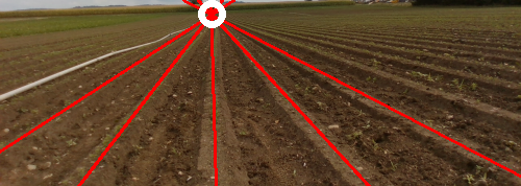
\includegraphics[width=0.75\textwidth]{Report/images/VPdetected.png}
   \caption{Vanishing Point detected}
   \label{pics:VPillu}
\end{figure}

This step makes sure that the lines in camera coordinates detected using the Hough transform all go towards the vanishing point, representing parallel lines in the world coordinates.\\

It is worth noting that the calculation of the vanishing point could in the future be used for other tasks, such as camera calibration, depth estimation, and perspective distortion correction. \\ 

\begin{figure}[H]
   \centering
   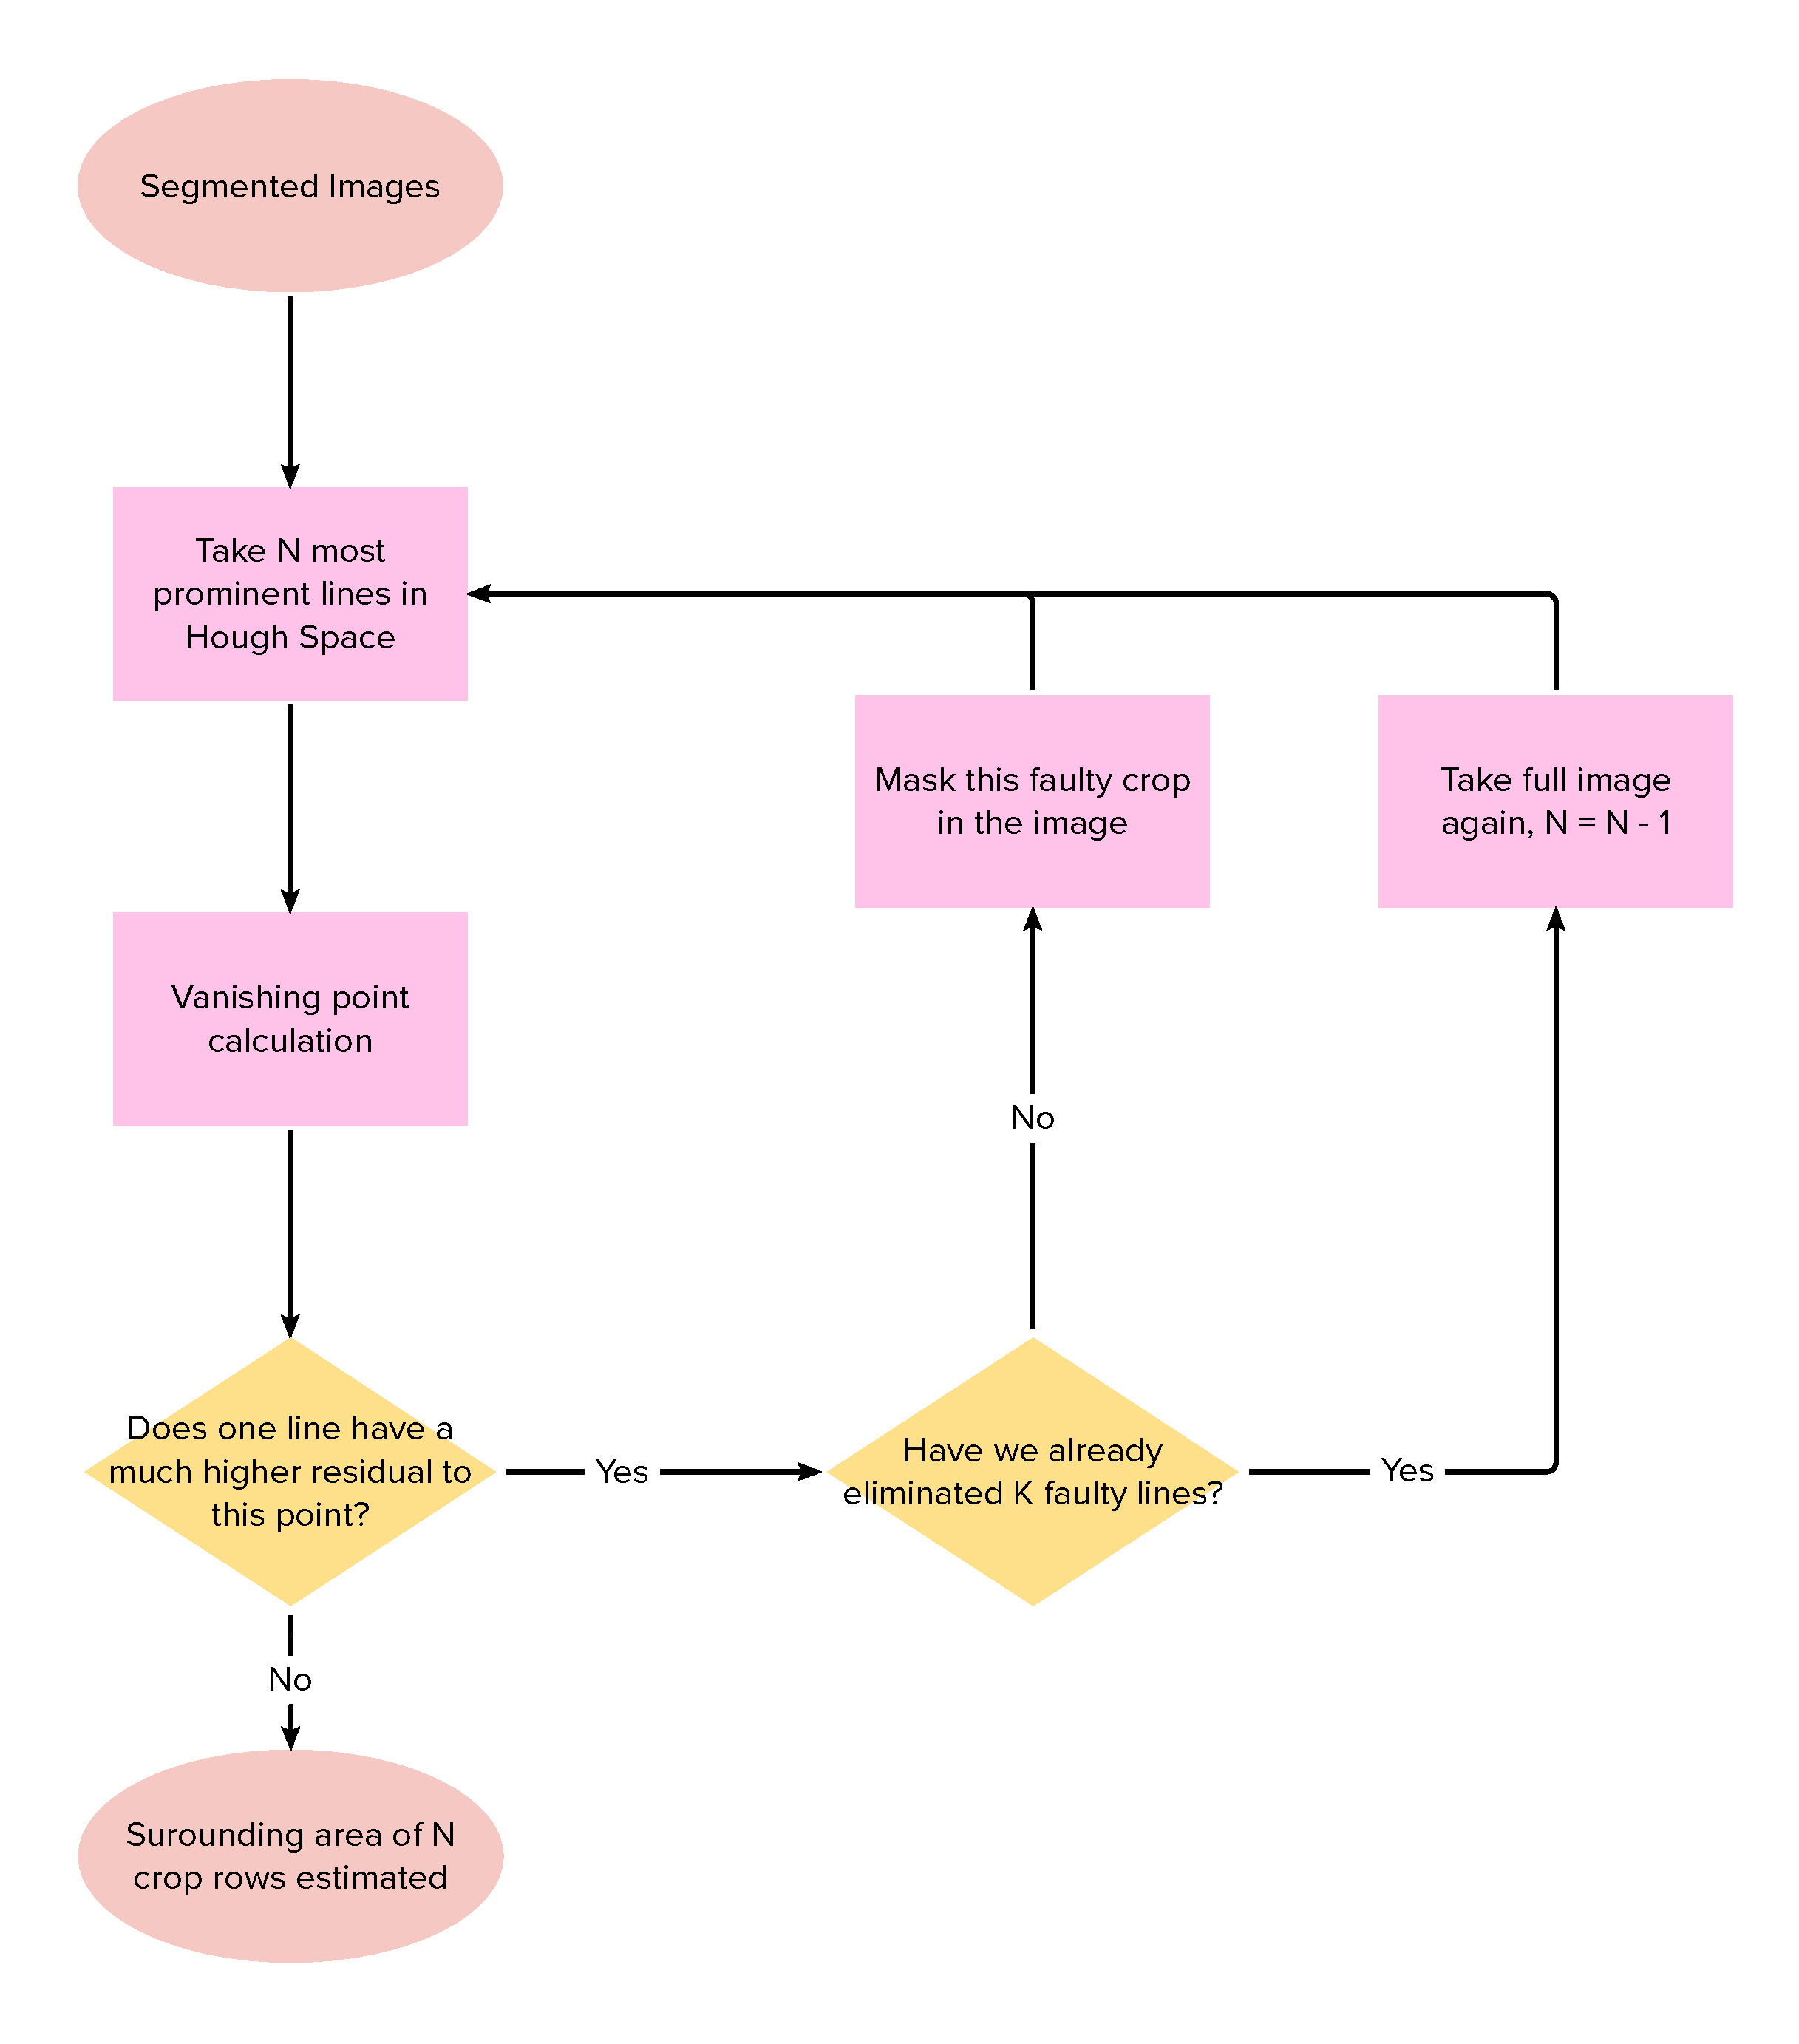
\includegraphics[width=0.75\textwidth]{Report/images/FlowCharts/VP calculation algorithm_2023-01-16_13-54-35.pdf}
   \caption{Flowchart of the Hough Process and Vanishing Point Calculation}
   \label{pics:VPCALC}
\end{figure}

Here, as it was proposed in \cite{CPCalcinHS}, the vanishing point is determined in the Hough Space and a iterative process is set up to eliminate outlier lines.  \\

As mentioned before, a point in the plane image is represented by a sinusoidal in the Hough space, which corresponds to all possible lines that could pass through this point. Thus, all the parallel lines in the world which pass through the vanishing point in the image plane should be on the same sinusoidal in the Hough space. Finding this sinusoidal should therefore describe the vanishing point in the following way:

\begin{equation}
\rho(\theta) = x_{0} \cdot \cos{\theta} + y_{0} \cdot \sin{\theta} = P(x_{0}, y_{0},\Phi) \cdot \sin{\theta + \Phi(x_{0}, y_{0})} .
 	\label{eq:my_equation}
\end{equation}

with : 
\begin{equation}
\begin{cases} 
P = x_{0}\cos(\Phi) \cdot \sin(1 + y_{0}^2/x_{0}^2) \\
\Phi = \arctan{y_{0}/x_{0}}
\end{cases}
 	\label{eq:my_equation}
\end{equation} \\

In the developed algorithm, a deterministic method is obviously not enough, as all parallel lines in the real world do not cross exactly at a single point, and as there could be "outlier" lines, not corresponding to parallel crops in the real world. The following statistical method was thus used :  


\begin{enumerate}
  \item Extract the dominant sinusoidal in the Hough space to get a first estimate of the vanishing point. This is done by solving the following minimisation problem : 
  
  \begin{equation}
\min_{x_{0}, y_{0}} \sum_{i=1}^{n} W_{i}(\rho_{i} - x_{0} \cos(\theta_{i}) - y_{0} \sin(\theta_{i}))^2
 	\label{eq:my_equation}
\end{equation}

Solving it leads to: 


\begin{equation}
  D_{it} =
    \begin{cases}
    A x_0 + C y_0 = D \\
    C x_0 + B y_0 = E
    \end{cases}       
\end{equation}

with : 
\begin{equation}
    \begin{cases}
      A = \sum_{i=1}^{n} W_{i} \cdot \cos{\theta_{i}}^2 \\
      B = \sum_{i=1}^{n} W_{i}\cdot  \sin{\theta_{i}}^2 \\
      C = \sum_{i=1}^{n} W_{i} \cdot \sin{\theta_{i}} \cdot \cos{\theta_{i}} \\
      D = \sum_{i=1}^{n} W_{i} \cdot \rho_i \cdot \cos{\theta_{i}}     \\
      E = \sum_{i=1}^{n} W_{i} \cdot \rho_i \cdot \sin{\theta_{i}}   \\

      \end{cases}
\end{equation}

  \item Once this point is found, compute the total variance of all lines with respect to this point : 
\begin{equation}
    \sigma^2 = \sum_{i=1}^{n} W_{i}  \epsilon_i^2
\end{equation}
    with : %TODO : rho en gras!!
\begin{equation}
    \epsilon_i =  \boldsymbol{\rho} -  \overline{\rho_{i}} 
\end{equation}

  
  \item If one of the lines is much more distant than this variance, that is \(\epsilon>k* \sigma\), classify it as an outlier and remove it from the detected line lists. An example of such a line is shown in Fig. \ref{pics:outlier}
  \item If more than k lines have already been detected as outliers, start detecting N-1 lines.
  \item Repeat the process: take the next dominant line in Hough space if N is unchanged, use the new set of lines to recalculate the vanishing point, and eliminate more outliers if necessary. 
  \item Stop when no more outliers are detected.

\end{enumerate}

A more concise explanation of this part can be visualized in Fig. \ref{pics:VPCALC}


\begin{figure}[H]
   \centering
   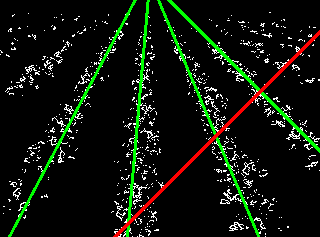
\includegraphics[width=0.65\textwidth]{Report/images/outlierdetected.png}
   \caption{Outlier line detected, soon to be eliminated}
   \label{pics:outlier}
\end{figure}





\section{Final detection : constrained RANSAC}
\label{sec:gliederung}

Once the estimate of the crop row position is estimated with the Hough transform and the vanishing point is calculated, RANSAC is used to fit lines in the center of the crop rows. Each fitted line uses a masked version of the vegetation segmented image, where only the regions surrounding the previously detected lines are kept, as shown in Fig. \ref{pics: Ransacmasking2}. \\

\begin{figure}[H]
\centering
\begin{subfigure}{0.3\textwidth}
    
\includegraphics[width=\textwidth]{Report/images/VEGSEG.png}
    \caption{Vegetation image}
    \label{fig:first}

\end{subfigure}
\begin{subfigure}{0.3\textwidth}%
    
\includegraphics[width=\textwidth]{Report/images/CROPMASK.png}
    \caption{Mask used}
    \label{fig:second}

\end{subfigure}
\begin{subfigure}{0.3\textwidth}%
    
\includegraphics[width=\textwidth]{Report/images/VEGCROPSEG.png}
    \caption{Segmented crop row}
    \label{fig:third}

\end{subfigure}

\caption{Segmentation of a single crop row}
\label{pics: Ransacmasking2}

\end{figure}



In this project, two approaches were tried to fit the rows with RANSAC : 


\begin{itemize}
  \item Fit all the crops at once, with a hard constraint on the vanishing point. All the lines had to pass through a same point, taken from the domain surrounding the region of the vanishing point previously calculated. The second points of the different lines used for line fitting were taken from the surroundings of the lines previously detected with the Hough transform. As a personalized Python version of the RANSAC function was used, the process took a lot of time.
  
  \item Fit single crop sequentially around the surrounding region of a line detected with the Hough transform, with a heavy bias towards the vanishing point - for this, the data points used for fitting a single line are augmented with multiple times the vanishing point coordinates - this method was selected for the final process, as it was faster and gave similar results.
\end{itemize}

There are two benefits to using RANSAC instead of the Hough transform :
\begin{enumerate}
  \item Hough transform is too slow for real-time application, using RANSAC on most frames and Hough only when necessary speeds up the crop row detection process. 
  \item The lines fitted with the Hough Algorithm are not necessarily the centers of the crops : when working with the edges of the image, they will even be fitted to the side of the crops. The data used for RANSAC being selected randomly from all the points of the crops, the lines detected are likely to be the center of the crops. 
\end{enumerate} 


\begin{figure}[H]
\centering
\begin{subfigure}{0.49\textwidth}
    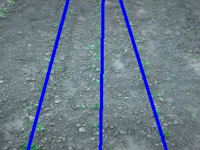
\includegraphics[width=\textwidth]{Report/images/houghdetection.png}
    \caption{Hough detection process, lines not fitted in the center }
    \label{fig:first}
\end{subfigure}
\begin{subfigure}{0.49\textwidth}%
    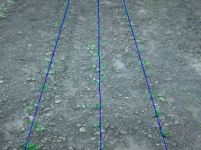
\includegraphics[width=\textwidth]{Report/images/ransacdetection.png}
    \caption{Ransac detection process, lines centered on the crops}
    \label{fig:second}
\end{subfigure}

\caption{Comparaison Hough and Ransac Process}
\end{figure}
\label{pics: HoughVSRansac}





 








\cleardoublepage
\chapter{Evaluation}

\section{Datasets Used}
\label{sec:gliederung}

To evaluate the developed algorithm, two datasets were used:

\begin{itemize}
  \item The Crop Row Benchmark Dataset (CRBD)  \cite{CRBD} is a collection of images featuring various types of crops that can be used to evaluate crop row detection methods. The dataset includes pictures of crops such as maize, celery, potato, onion, sunflower, and soybeans, with varying levels of weeds and shadows. Some images also contain elements such as grass, sky, or roads. The images were taken at different angles and captured using a Panasonic LUMIX DMC-F2 digital camera in the spring of 2014 in the Croatian region of Slovenia. The dataset has a total of 281 images, including 47 images of straight crop rows, which are the main focus of interest of this project.

  
  \item Caterra's own dataset, taken with its front camera intel realsense d435i. It was used to evaluate the algorithm on time-related frames. For this data set that contains no ground truth, a simple visual validation was conducted. 
\end{itemize}

It is important to point out that further evaluations should be conducted on the algorithm, especially to evaluate it on video and later to use it in real time. 
Weather conditions such as rain, snow, and heavy mist were not evaluated as not part of any dataset. 

\section{Results on the Crop Row Benchmark Dataset}
\label{sec:gliederung}

\subsection{Evaluation Method}
\label{sec:gliederung}

To compare the results obtained against the ground truth, two matrices are constructed, one for the ground truth and one for the algorithm developed. In this matrix, the number of rows corresponds to the number of image rows (h), and each row of the matrix has m elements, represented by the horizontal coordinates of m adjacent crop rows detected by the method considered in the v-th image row. 
To compute the accuracy, we use the CRDA formula defined in \cite{8730214} as:


\begin{equation}
CRDA = \frac{1}{m*(h-v_0)} \sum_{v=v_{0}}^{h-1} \sum_{i=1}^{m} s(u_{v,i}^{\ast}, u_{v,i}, d_{v}^{\ast})
 	\label{eq:my_equation}
\end{equation}

with : 
\begin{equation}
s(u^{\ast}, u, d^{\ast}) = max\left(1-\left(\frac{u^{\ast}-u}{\sigma d}\right)^{2}, 0\right)
 	\label{eq:my_equation}
\end{equation}

\newenvironment{conditions*}
  {\par\vspace{\abovedisplayskip}\noindent
   \tabularx{\columnwidth}{>{$}l<{$} @{}>{${}}c<{{}$}@{} >{\raggedright\arraybackslash}X}}
  {\endtabularx\par\vspace{\belowdisplayskip}}

\begin{eqexpl}[5mm]
\item{$m$}{number of crops to be detected}
\item{$v_0$}first line where evaluation starts (could be bushy with undefined crop position on top of image)
\item{$h$}height of the image
\item{$u^{\ast}$}ground truth on line v
\item{$u$}{personal results on line v}
\item{$\sigma$}user defined parameter that is set based on the accuracy needed: in the following evaluation, it is set to 0.3, which means that the matching score is greater than zero only if the horizontal distance between a detected crop row and the corresponding ground truth curve is less than 30\% of the distance between adjacent crop rows
\item{$d^{\ast}$}distance between crops in ground truth
\end{eqexpl}


\subsection{Results}
\label{sec:gliederung}

Our algorithm achieved a median CRDA of 0.816. 
Some examples of detected crop rows and their score are shown in Fig. \ref{pics:resultsdiffcroprow}. %PB HERE
The algorithm presents better results for less bushy crop rows, as when bushes are too present, the Hough transform has many lines to choose from. When weeds are far too present in the center of the crop rows, the algorithm may detect an extra row - this is hopefully not the case if an agricultural robot passes regularly. It is also worth noting that some of the crops from the CRDA images are indistinguishable even from the human eye. \\

Despite the high level of accuracy, the current computational time of the algorithm is too high to be implemented in real-time applications. While the images process using sanely the RANSAC were computed in milliseconds, the average time to process an image using the Hough Transform was 10 seconds. Depending on the accuracy image, this transform can be performed very regularly, which is not practical for real-time applications. As a future work,
it would be important to optimize the algorithm's computational time, to enhance the possibility of using it in real-time applications.

\begin{table}[h]
\begin{center}
 \label{tab:tabnefz}
 \begin{tabular}{|l|l|l|l|l}
 \hline
 Datasets & Mean & Median \\ \hline \hline
 All Crop Rows & 0.773 & 0.816 \\
 Non bushy crop rows & 0.821 & 0.856  \\
 Bushy crop row & 0.625 & 0.689 \\
 \hline
 \end{tabular}
\end{center}
 \caption{Results on the CRBD}\vspace{1ex}

\end{table}


\begin{figure}[H]
\centering
\begin{subfigure}{0.49\textwidth}
    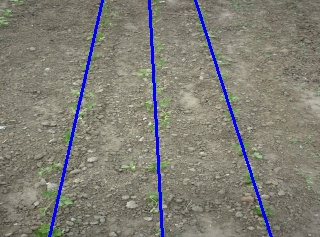
\includegraphics[width=\textwidth]{Report/images/ransac001.jpg}
    \caption{CRDA score of 0.952}
    \label{fig:first}
\end{subfigure}
\begin{subfigure}{0.49\textwidth}%
    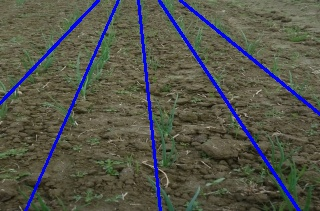
\includegraphics[width=\textwidth]{Report/images/ransac002.jpg}
    \caption{CRDA score of 0.853}
    \label{fig:second}
\end{subfigure}
\begin{subfigure}{0.49\textwidth}%
    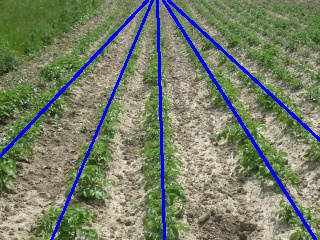
\includegraphics[width=\textwidth]{Report/images/ransac008.jpg}
    \caption{CRDA score of 0.797}
    \label{fig:third}
\end{subfigure}
\begin{subfigure}{0.49\textwidth}%
    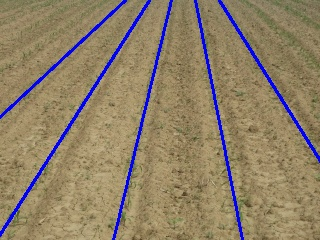
\includegraphics[width=\textwidth]{Report/images/ransac095.jpg}
    \caption{CRDA score of 0.984}
    \label{fig:third}
\end{subfigure}
\caption{Results of the algorithm on different types of crop rows}
\label{pics:resultsdiffcroprow}
\end{figure}

\section{Results on Caterra's dataset}

The Rosbag was captured using the rover's front camera, a realsense d435i.  
The Rosbag contained 776 images of the rover advancing in the field. For visualization, the annotated video can be seen here : \url{https://youtu.be/yA1oaAT4Wgg}.

Depending on the accuracy needed, the number of frames before recalculating the Hough transform and the vanishing point varies. For the visualized video, we have chosen $K=5$.

Crops are detected accurately most of the time, and when an error occurs, it is quickly corrected by the algorithm when this one recalculates the hough transform.

\begin{figure}
\centering
\begin{subfigure}{0.49\textwidth}
    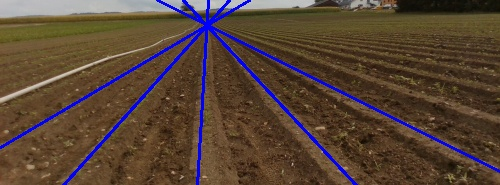
\includegraphics[width=\textwidth]{Report/images/rgb000.jpg}
    \label{fig:first}
\end{subfigure}
\begin{subfigure}{0.49\textwidth}
    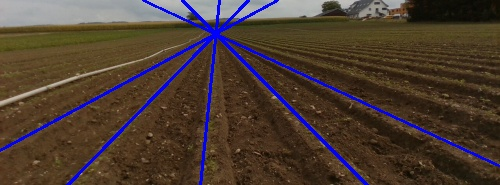
\includegraphics[width=\textwidth]{Report/images/rgb200.jpg}
    \label{fig:first}
\end{subfigure}
\begin{subfigure}{0.49\textwidth}
    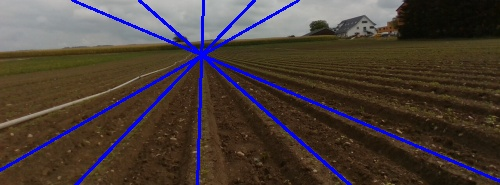
\includegraphics[width=\textwidth]{Report/images/rgb400.jpg}
    \label{fig:first}
\end{subfigure}
\begin{subfigure}{0.49\textwidth}
    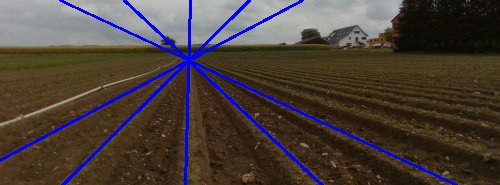
\includegraphics[width=\textwidth]{Report/images/rgb600.jpg}
    \label{fig:first}
\end{subfigure}
\caption{Annotated frames 0, 200, 400, and 600 of the dataset}
\end{figure}

\cleardoublepage
\chapter{Discussion}

\section{Failure cases}

As the algorithm focuses on fitting straight lines, more work is needed to detect curved crop rows (Fig. \ref{fig:cropcurved}). The Hough and RANSAC processes should be adapted to use customs models, not just linear models. This would mean complications when it comes to the detection of vanishing points and thus for outlier elimination.

Another issue is the non-ordered detection of the lines : since the lines are detected by order of prominence, the first line is not necessarily the most centered one. This can be a problem if a large number of lines is present in a picture : a central row may not be part of the main N rows and is only detected when we adjust the number of crop to be detected (as shown in Fig. \ref{fig:missedcrop})
This problem has many solutions : as crops are set in an equidistant way, the distance between two crop rows could be used as an extra constraint. An easier solution would be to perform a search in the middle of two rows when their distance has a high deviation from the average distance between rows in a picture.

Finally, in some extreme cases where bushes are too prominent, the Hough transform detects too many faulty lines and does not manage to calculate a correct vanishing point. The lines kept as "inliers" are the faulty ones.

\begin{figure}[H]
\centering
\begin{subfigure}
    {0.3\textwidth}
    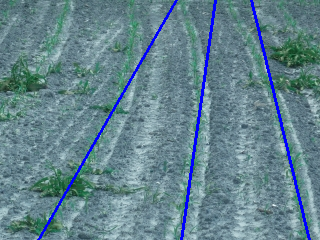
\includegraphics[width=\textwidth]{Report/images/FailureCases/img annotated_ _screenshot_07.01.2023 (2).png}
    \caption{Curved crop rows}
    \label{fig:cropcurved}
\end{subfigure}
\begin{subfigure}{0.3\textwidth}%
    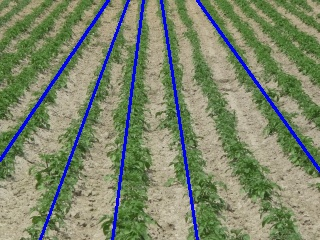
\includegraphics[width=\textwidth]{Report/images/ransaccropskipped.jpg}
    \caption{Wrong order detection}
    \label{fig:missedcrop}

\end{subfigure}
\begin{subfigure}{0.3\textwidth}%
    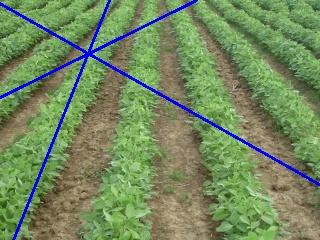
\includegraphics[width=\textwidth]{Report/images/faultyransac.jpg}
    \caption{Bushy crop rows}
    \label{fig:missedcrop}

\end{subfigure}
\end{figure}
\label{pics: bushyremoval}






\section{Future Work}

We have successfully developed an algorithm that detects crop rows in an RGB image or video with high accuracy. Nevertheless, improvements could be made and different cases could be taken into account. 

\begin{enumerate}
    \item Computational time : currently, the algorithm is too slow for real-time applications. A more efficient image processing technique and parallel processing could be implemented. 
    \item Prior information : Our algorithm could be made even more robust by integrating more prior information, such as the distance between crop rows or the number of crop rows
    \item Sensors fusion : integrating
    additional sensors, such as LiDAR, would enhance the algorithm's accuracy
    \item Deep Learning : for even better crop row detection or vegetation segmentation, deep learning could be added
    \item Camera Calibration: The algorithm assumes that the camera is
    calibrated, which means that the intrinsic and extrinsic parameters of
    the camera are known. However, in real-world applications, the camera
    may not be calibrated, or the calibration may drift over time.
    Therefore, it would be beneficial to include an automatic camera
    calibration module to the algorithm to improve its robustness. \\
\end{enumerate}

Of course, the main reason for crop row detection is the navigation of the rover : path planning is another important aspect to consider. This project has concentrated on detecting crop rows and does not provide
information about the optimal path for the robot to follow. This path could be generated using techniques such 
as the A* algorithm, Voronoi diagrams, or other known path planning
techniques to ensure that the robot can navigate efficiently and safely between detected crops. \\

It is also important to note that the dataset used is not representative of all crops: different data sets should be collected to better measure the degree to which the algorithm stays accurate.


\chapter{Conclusion}

In conclusion, the crop row detection algorithm developed in this report utilizes simple image processing techniques such as color clustering, vanishing point calculation, the Hough transform, and RANSAC. \\

The algorithm is robust to different illuminations, growth stages, and points of view. Since simple computer vision techniques were used, it is also generalizable and is not limited to a single type of plant. \\

The algorithm was found to be accurate for straight crop rows, especially for images with low to medium vegetation density. It achieved a median accuracy of 82\% when tested on a dataset of various images, demonstrating its effectiveness in detecting crop rows in images.  \\

In the future, this algorithm could be further improved by using additional techniques such as machine learning and deep learning models, or LiDAR for very bushy regions. Overall, the algorithm shows promise in being a useful tool for precision agriculture and crop monitoring, but further optimization is needed to make it real-time.
\cleardoublepage

% \input{}
% \cleardoublepage
% \input{}
% \cleardoublepage
% ...
%

%%%%%%%%%%%%%%%%%%%%%%%%%%%%%%%%%%%%%%%%%%%%%%%%%%%%%%%%%%%%%%%%%%%%%%%%%%%%%%%
% Bibliography
%%%%%%%%%%%%%%%%%%%%%%%%%%%%%%%%%%%%%%%%%%%%%%%%%%%%%%%%%%%%%%%%%%%%%%%%%%%%%%%
\chapter*{Acknowledgement}
\addcontentsline{toc}{chapter}{Acknowledgement}


I would like to thank my supervisors Patrick Barton and Cornelius von Einem for their guidance and support throughout my Master's semester project. I am grateful for their mentorship, their time and their expertise.


\cleardoublepage
\bibliographystyle{bibliography/IEEEtranN}
\bibliography{bibliography/references}
\addcontentsline{toc}{chapter}{Bibliography}
\cleardoublepage

%%%%%%%%%%%%%%%%%%%%%%%%%%%%%%%%%%%%%%%%%%%%%%%%%%%%%%%%%%%%%%%%%%%%%%%%%%%%%%%
% Appendix
%%%%%%%%%%%%%%%%%%%%%%%%%%%%%%%%%%%%%%%%%%%%%%%%%%%%%%%%%%%%%%%%%%%%%%%%%%%%%%%
%\appendix
\chapter{Appendix - Hyperparameters }\label{sec:irgendwas}

\begin{table}[h]
\begin{tabularx}{\textwidth}{|>{\hsize=0.5 \hsize}X
                                |>{\hsize=0.5 \hsize}X
                                |>{\hsize=2 \hsize}X|}
% \begin{center}

 % \label{tab:tabnefz}
 %\begin{tabularx}{\textwidth}{ |l|X| }
 % \begin{tabular}{|l|l|l|l|l}
 \hline
 Parameters & Values & Description \\ \hline \hline
 N & 5 & Default number of crop row to be detected \\
  \hline

 K & 5 & Default number of frame before executing the complete Hough Transform Process  \\
  \hline

 r & 0.1 & Ratio vegetatative pixels/non vegetation pixels of the image to be considered "bushy" \\
  \hline

 $\sigma$ & 0.3 & User defined parameter based on the accuracy needed for the CRDA \\
  \hline

 bw & 0.35 & Fraction of the bandwidth used for creating the mask over the width of the image  \\
  \hline

 $\alpha$ & 0.2 & Minimum angle for crop row to not be considered as the horizon [rad]\\
  \hline

 $\beta$ & 0.1 & Difference minimum between angles of two different crop row [rad] \\
  \hline

 tol & 6 & Color clustering tolerance for different color to be clustered together \\
  \hline

 
 lim & 6 & Maximum number of color clustered \\
  \hline

 k & 4 & Initial tolerance in vegetation segmentation - pixels within a color difference in norm of k to the vegetation color will be considered vegetation pixels  \\
  \hline

 $it_{max}$ & 5 & If $it_{max}$ outlier line were detected in a row, the algorithm start detecting $N-1$ lines \\
  \hline

 var & 1.25 & Maximum ratio difference between the distance of an inlier line to the vanishing point and the standard deviation  \\

 \hline

\end{tabularx}
%  \end{tabular}
% \end{center}
 \caption{Hyperparameters used throughout the algorithm}
\label{appendix:hyperparam}
\end{table}
%\cleardoublepage
%\chapter{Datasheets}\label{sec:datasheets}

\includepdf[scale=0.75]{images/datasheets.pdf}

\end{document}